\documentclass{article}
\usepackage[sexy, hdr, fancy]{evan}
\usepackage{graphicx}
\graphicspath{.}
\setlength{\droptitle}{-4em}

\DeclareMathOperator{\re}{Re}
\DeclareMathOperator{\im}{Im}

\lhead{Homework 1}
\rhead{Complex Analysis}
\lfoot{}
\cfoot{\thepage}

\begin{document}
\title{Homework 1}
\maketitle
\thispagestyle{fancy}

\section*{Section 1.1}

\begin{itemize}
	\item[8.] Write the number in the form $a+bi.$
		\begin{align*}
			\frac{(8+2i)-(1-i)}{(2+i)^2}
		\end{align*}
		\begin{soln}
			\begin{align*}
				\frac{(8+2i)-(1-i)}{(2+i)^2} &= \frac{(7+3i)(2-i)^2}{(2+i)^2(2-i)^2} = \frac{(7+3i)(3-4i)}{(2^2+1^2)^2} \\
				&= \frac{33-19i}{(4+1)^2} = \boxed{\frac{33}{25} - \frac{19}{25}i}
			\end{align*}
		\end{soln}

	\item[10.] Write the number in the form $a+bi.$
		\begin{align*}
			\left[ \frac{2+i}{6i-(1-2i)} \right]^2
		\end{align*}
		\begin{soln}
			\begin{align*}
				\left[ \frac{2+i}{6i-(1-2i)} \right]^2 &= \left( \frac{2+i}{-1+8i} \right)^2 = \frac{(2+i)^2(-1-8i)^2}{(-1+8i)^2(-1-8i)^2} \\
				&= \frac{(3+4i)(-63+16i)}{(1^2+8^2)^2} = \frac{-253-204i}{65^2} = \boxed{-\frac{253}{4225} - \frac{204}{4225}i}
			\end{align*}
		\end{soln}

\end{itemize}

\section*{Section 1.2}

\begin{itemize}
	\item[7.] (e) Describe the set of points $z$ in the complex plane that satisfies $\abs{z}=\re z+2.$
		\begin{soln}
			Let $z=a+bi,$ Then we have
			\begin{align*}
				\abs{z} &= \abs{a+bi} = \sqrt{a^2+b^2} \\
				\re z + 2 &= a+2 \\
				\implies \sqrt{a^2+b^2} &= a+2 \implies a^2+b^2 = a^2+4a+4 \\
				\implies b^2&=4a+4 \implies a = \frac{1}{4} b^2-1
			\end{align*}
			This traces out a parabola in the complex plane. 
		\end{soln}

	\item[16.] Prove that if $\abs{z}=1$ ($z\neq 1$), then $\re[1/(1-z)]=\frac{1}{2}.$
		\begin{proof}
			Let $z=a+bi.$ Then we have $\abs{z}=\abs{a+bi}=\sqrt{a^2+b^2}=1\implies a^2+b^2=1.$ Then
			\begin{align*}
				\re \left( \frac{1}{1-z} \right) &= \re \left( \frac{1}{1-a-bi} \right) = \re\left[ \frac{(1-a)+bi}{(1-a-bi)(1-a+bi)} \right] \\
				&= \re \left[ \frac{1-a+bi}{(1-a)^2+b^2} \right] = \frac{1-a}{1-2a+a^2+b^2} \\
				&= \frac{1-a}{1-2a+1} = \frac{1-a}{2-2a} = \frac{1}{2}
			\end{align*}
			as desired.
		\end{proof}
		
\end{itemize}

\section*{Section 1.3}

\begin{itemize}
	\item[5.] (d) Find the value of
		\begin{align*}
			\abs{\frac{(\pi+i)^{100}}{(\pi-i)^{100}}}
		\end{align*}
		\begin{soln}
			Let $z=\pi+i.$ Then we have
			\begin{align*}
				\abs{\frac{z^{100}}{(\overline z)^{100}}} &= \frac{\abs{z}^{100}}{\abs{\overline z}^{100}} = \left( \frac{\abs{z}}{\abs{\overline z}} \right)^{100} = \boxed{1}
			\end{align*}
		\end{soln}

	\item[7.] (h) Find the argument of this complex number and write it in polar form. 
		\begin{align*}
			\frac{-\sqrt{7}(1+i)}{\sqrt{3}+i}
		\end{align*}
		\begin{soln}
			We have
			\begin{align*}
				\frac{-\sqrt{7}(1+i)}{\sqrt{3}+i} &= \frac{-\sqrt{7}(1+i)(\sqrt{3}-i)}{3+1^2} = \frac{-\sqrt{7}\left[ (1+\sqrt{3})+(\sqrt{3}-1)i \right]}{4} \\
				&= \frac{-\sqrt{7}-\sqrt{21}}{4} + \frac{\sqrt{7}-\sqrt{21}}{4}i
			\end{align*}
			Now, we have
			\begin{align*}
				\theta &= \tan\inv\left( \frac{\sqrt{7}-\sqrt{21}}{-\sqrt{7}-\sqrt{21}} \right) = \tan\inv(2-\sqrt{3}) = \frac{\pi}{12} \\
				r &= \sqrt{\left( \frac{-\sqrt{7}-\sqrt{21}}{4} \right)^2 + \left( \frac{\sqrt{7}-\sqrt{21}}{4} \right)^2} = \frac{\sqrt{14}}{2}
			\end{align*}
			Since this lies in the third quadrant, we adjust to get $\theta_0=-\frac{11\pi}{12},$ so the polar form is $\boxed{\frac{\sqrt{14}}{2}\cis\left( -\frac{11\pi}{12} \right).}$
		\end{soln}

	\item[28.] Let the crankshaft pivot $O$ lie at the right of the origin of the coordinate system, and let $z$ be the complex number giving the location of the base of the piston rod, as depicted in Fig 1.14,
		\begin{align*}
			z=\ell+id
		\end{align*}
		where $\ell$ gives the piston's linear excursion and $d$ is a fixed offset. The crank arm is described by $A=a(\cos \theta_1+i\sin\theta_1)$ the connecting arm by $B=b(\cos\theta_2+i\sin\theta_2)$ ($\theta_2$ is negative in Fig 1.14). Exploit the obvious identity $A+B=z=\ell+id$ to derive the expression relating the piston position to the crankshaft angle:
		\begin{align*}
			\ell=\cos\theta_1+b\cos\left[ \sin\inv\left( \frac{d-a\sin\theta_1}{b} \right) \right]
		\end{align*}
		\begin{soln}
			Because of the identity
			\begin{align*}
				A+B &= a(\cos\theta_1+i\sin\theta_1)+b(\cos\theta_2+i\sin\theta_2) \\
				&= (a\cos \theta_1+b\cos\theta_2) + i(a\sin\theta_1+b\sin\theta_2) \\
				&= \ell+id
			\end{align*}
			we must have 
			\begin{align*}
				a\cos\theta_1+b\cos\theta_2 &= \ell \\
				a\sin\theta_1+b\sin\theta_2 &= d \implies \theta_2 = \sin\inv\left( \frac{d-a\sin\theta_1}{b} \right) \\
				\implies \ell &= a\cos \theta_1 + b\cos\left[ \sin\inv\left( \frac{d-a\sin\theta_1}{b} \right) \right]
			\end{align*}
			as desired.
		\end{soln}
		
\end{itemize}

\section*{Section 1.4}

\begin{itemize}
	\item[11.] Determine which of the following properties of the real exponential function remain true for the complex exponential function
		\begin{enumerate}[(a)]
			\item $e^x$ is never zero.
				\begin{answer*}
					This is true.
				\end{answer*}

			\item $e^x$ is a one-to-one function.
				\begin{answer*}
					This is false. We have $1=e^{0}=e^{2\pi i}.$
				\end{answer*}

			\item $e^x$ is defined for all $x.$
				\begin{answer*}
					This is true.
				\end{answer*}

			\item $e^{-x}=1/e^x.$
				\begin{answer*}
					This is true.
				\end{answer*}
				
		\end{enumerate}

		\newpage
	\item[18.] Sketch the curves that are given for $0\le t\le 2\pi$ by
		\begin{enumerate}[(a)]
			\item $z(t)=e^{(1+i)t}$ 
				\begin{answer*}
					Plots all created in MATLAB.

					This is $e^{(1+i)t} = e^t e^{it} = e^t \cos t + i e^t\sin t,$ so we may model this parametrically in $\RR^2.$
					\begin{figure}[h!]
						\centering
						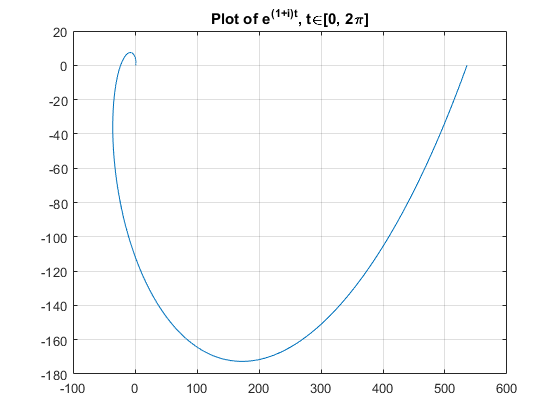
\includegraphics[width=10cm]{18a.png}
						\caption{Plot of $e^{(1+i)t}, t\in[0, 2\pi]$}
					\end{figure}
				\end{answer*}
				
			\item $z(t)=e^{(1-i)t}$ 
				\begin{answer*}
					Similar to above, $e^{(1-i)t} = e^t e^{-it} = e^t \cos (-t) + i e^t\sin (-t)=e^t \cos t - ie^t\sin t.$
					\begin{figure}[h!]
						\centering
						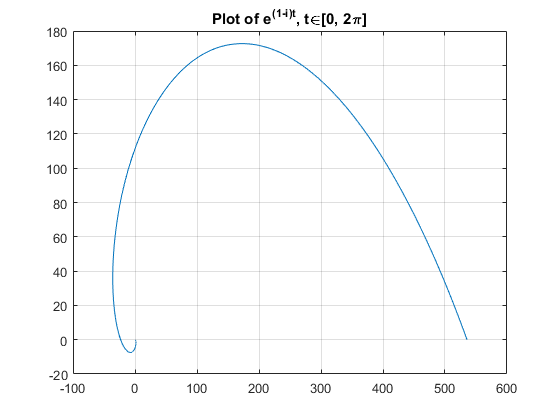
\includegraphics[width=10cm]{18b.png}
						\caption{Plot of $e^{(1-i)t}, t\in[0, 2\pi]$}
					\end{figure}
				\end{answer*}
				\newpage

			\item $z(t)=e^{(-1+i)t}$
				\begin{answer*}
					Similar to above, $e^{(-1+i)t} = e^{-t} e^{it} = e^{-t} \cos t + i e^{-t}\sin t.$
					\begin{figure}[h!]
						\centering
						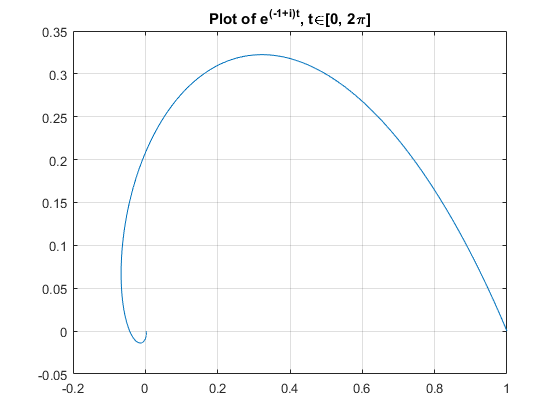
\includegraphics[width=10cm]{18c.png}
						\caption{Plot of $e^{(-1+i)t}, t\in[0, 2\pi]$}
					\end{figure}
				\end{answer*}

			\item $z(t)=e^{(-1-i)t}$
				\begin{answer*}
					Similar to above, $e^{(-1-i)t} = e^{-t} e^{-it} = e^{-t} \cos t - i e^{-t}\sin t.$
					\begin{figure}[h!]
						\centering
						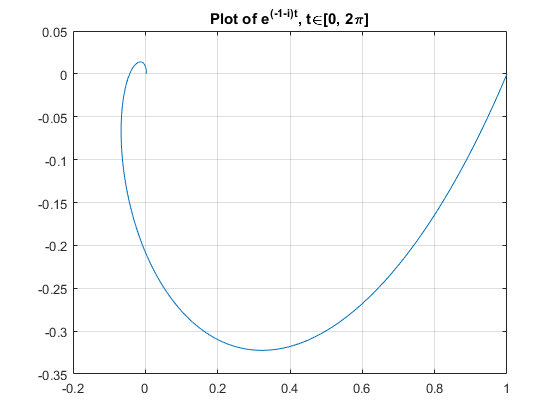
\includegraphics[width=10cm]{18d.png}
						\caption{Plot of $e^{(-1-i)t}, t\in[0, 2\pi]$}
					\end{figure}
				\end{answer*}
				
		\end{enumerate}

		\newpage
	\item[22.] Show that if $n$ is an integer then
		\begin{align*}
			\int_0^{2\pi} e^{in\theta}\, d\theta = \int_0^{2\pi}\cos(n\theta)\, d\theta + i\int_0^{2\pi}\sin(n\theta)\, d\theta = \begin{cases}
				2\pi & \text{if }n=0 \\
				0 &\text{if }n\neq 0
			\end{cases}
		\end{align*}
		\begin{proof}
			We have $e^{in\theta}=\cos (n\theta) + i\sin(n\theta),$ so
			\begin{align*}
				\int_0^{2\pi} e^{in\theta}\, d\theta &= \int_0^{2\pi} \cos(n\theta)\, d\theta + i\int_0^{2\pi} \sin(n\theta)\, d\theta
			\end{align*}
			If $n=0,$ then this is
			\begin{align*}
				\int_0^{2\pi} \cos 0\, d\theta + i\int_0^{2\pi}\sin 0\, d\theta = \int_0^{2\pi}1\, d\theta + i\int_0^{2\pi} 0\, d\theta = 2\pi
			\end{align*}
			Otherwise, this is
			\begin{align*}
				\frac{1}{n}\sin(n\theta)\bigg\vert_0^{2\pi} - i\cdot \frac{1}{n}\cos(n\theta)\bigg\vert_0^{2\pi} = 0
			\end{align*}
		\end{proof}
		
\end{itemize}

\section*{Section 1.5}

\begin{itemize}
	\item[4.] Use the identity (1) to show that
		\begin{enumerate}[(a)]
			\item $(\sqrt{3}-i)^7=-64\sqrt{3}+64i$
				\begin{soln}
					\begin{align*}
						\sqrt{3}-i &= 2\left( \frac{\sqrt{3}}{2} - \frac{1}{2}i \right) = 2\left[ \cos\left( -\frac{\pi}{6} \right) + i\sin\left( -\frac{\pi}{6} \right) \right] \\
						\implies \left( \sqrt{3}-i \right)^7 &= 2^7 \left[ \cos \left( -\frac{7\pi}{6} \right) + i\sin\left( -\frac{7\pi}{6} \right) \right] = 128\left( -\frac{\sqrt{3}}{2} + \frac{1}{2}i \right) \\
						&= -64\sqrt{3} + 64i
					\end{align*}
				\end{soln}

			\item $(1+i)^{95}=2^{47}(1-i)$
				\begin{soln}
					\begin{align*}
						1+i &= \sqrt{2}\left( \frac{1}{\sqrt{2}} + \frac{1}{\sqrt{2}}i \right) = \sqrt{2}\left( \cos\frac{\pi}{4} + i\sin\frac{\pi}{4} \right) \\
						\implies (1+i)^{95} &= \sqrt{2}^{95}\left( \cos \frac{95\pi}{4} + i\sin\frac{95\pi}{4} \right) = 2^{47}\sqrt{2}\left( \frac{1}{\sqrt{2}} - \frac{1}{\sqrt{2}}i \right) \\
						&= 2^{47}(1-i)
					\end{align*}
				\end{soln}
				
		\end{enumerate}
		\newpage

	\item[5.] (f) Find the value of $\left( \frac{2i}{1+i} \right)^{1/6}$
		\begin{soln}
			\begin{align*}
				\frac{2i}{1+i} &= \frac{2i(1-i)}{1^2+1^2} = 1 + i = \sqrt{2}e^{i\pi/4} \\
				\implies \left( \frac{2\pi}{1+i} \right)^{1/6} &= 2^{1/12} \exp\left\{ i\left( \frac{\pi/4+2k\pi}{6}\right) \right\} = \boxed{2^{1/12}\exp\left\{ i\left( \frac{\pi}{24} + \frac{k\pi}{3} \right) \right\}, k\in\ZZ}
			\end{align*}
		\end{soln}

\end{itemize}

\end{document}
